\chapter{相关技术及研究现状}\label{chap:Relate}

本章节主要介绍SMT和非线性实数理论的相关基本概念以及研究现状。首先,本文给出SMT问题和非线性实数理论的语法,然后给出解空间表达以帮助读者更好理解SMT问题的本质。紧接着我们给出CDCL(T)算法的结构、MCSAT算法原理以及其他一些SMT求解器的介绍。然后我们给出近几年来局部搜索在SMT问题上的应用,包括线性整数逻辑、多线性逻辑和部分多项式理论等。最后,我们总结目前算法的缺点和非线性问题的挑战,并引出我们的工作带来的进展和突破。

\section{可满足性模理论与非线性实数问题}
首先,本文给出可满足行模理论(Satisfiability Modulo Theories, SMT)问题的一般定义,前置概念介绍如下:

\begin{definition}[\textbf{变量}]
SMT问题中的变量根据赋值要求分为布尔变量和算术变量。布尔变量是只能取布尔值($\top, \bot$)的变量,布尔变量集合一般用$B$表示。算术变量可以取整数或者实数值,一般用$R$表示。非线性实数问题中所有算术变量必须取实数值。
\end{definition}

\begin{definition}[\textbf{多项式约束}]
非线性问题主要由多项式约束构成,多项式约束的形式为$P(x) \sim 0$,其中$P(x)$是一个多项式,$\sim$是一个关系符号,可以是$=, <, >$中的一个。
\end{definition}


Tseitin编码保证了任意的逻辑约束可以在多项式时间内转化为合取范式(CNF)。为方便说明,本文中所有SMT约束表达成为CNF形式,一些基本概念如下:
\begin{definition}{\textbf{命题文字}}
命题文字(literal)是可满足问题中的基本结构,包括正文字($p$)和负文字($\neg p$)。非线性实数理论的命题文字一般是多项式约束或布尔变量约束。正文字只有当对应的多项式约束满足时才满足,负文字只有当对应的多项式约束不满足时才满足。一个典型的非线性实数文字比如$x^2 + y > 0$或者$\neg (x + y^3 < 0)$。
\end{definition}

\begin{definition}{\textbf{子句}}
子句(clause)定义为文字的析取结构,一般记为$C = l_1 \vee l_2 \vee \dots \vee l_n$,其中$l_i$是一个文字。当子句包含的所有文字不满足时子句不满足,只要有一个文字被满足子句也被满足。\textbf{空子句}一般表示不包含任何文字的子句。比如,一个非线性实数理论的子句形如$(x^2 + y > 0) \vee (x + y^3 < 0)$。
\end{definition}

\begin{definition}{\textbf{公式}}
公式(formula)定义为子句的合取结构,一般记为$\varphi = C_1 \wedge C_2 \wedge \dots \wedge C_m$,其中$C_i$是一个子句。当公式包含的所有子句都满足时公式满足,只要有一个子句不满足公式就不满足。一个非线性实数理论的公式比如$(x^2 + y > 0) \wedge (x + y^3 < 0)$。
\end{definition}


\begin{definition}{\textbf{赋值}}
赋值(assignment)指的是变量到布尔值或者实数的一种映射,布尔变量赋值为$f: B \rightarrow \{\top, \bot\}$,算术变量赋值为$f: R \rightarrow \mathbb{R}$。一个赋值$f$满足一个公式$\varphi$,记作$f \models \varphi$,当且仅当对于公式中的每一个子句$C_i$,至少有一个文字$l_j$满足$f \models l_j$。赋值可以分为部分赋值(partial assignment)和完全赋值(full assignment),部分赋值只对部分变量存在映射,完全赋值对所有变量都存在映射。赋值一般记为一组映射,比如$\{x \mapsto 2, y \mapsto 3\}$。
\end{definition}

\begin{definition}{\textbf{评估}}
评估(evaluation)指的是给定赋值和一个文字,判断当前文字是否满足,记为$eval (ass, l) \rightarrow \{\top, \bot\}$,其中$ass$是一个赋值,$l$是一个文字。评估的结果为$\top$表示文字满足,为$\bot$表示文字不满足。比如$eval (\{x \mapsto 2, y \mapsto 3\}, x^2 + y > 0) \rightarrow \top$。评估只有在文字包含的所有变量都有赋值时才有返回值。
\end{definition}

\begin{definition}{\textbf{可满足性模理论(SMT)}}
可满足性模理论(SMT)指的是给定一个逻辑公式$\varphi$,如果存在一组赋值$f$使得$f \models \varphi$,则称$\varphi$是\textbf{可满足的(satisfiable)},否则称$\varphi$是\textbf{不可满足的(unsatisfiable)}。SMT问题的目标是找到一个可满足的赋值,即找到一个满足公式的赋值,或者证明赋值不可满足。
\end{definition}

我们给出以下例子\ref{ex:SMT}进一步说明SMT问题的可满足性。

\begin{example}
\label{ex:SMT}
给定SMT公式$\varphi = (x^2 + y > 0) \wedge (x + y^3 < 0)$,我们可以找到一组赋值$f = \{x \mapsto 2, y \mapsto -2\}$使得$f \models \varphi$。因此我们称该问题是可满足的。给定SMT公式$\varphi = (x^2 + y^2 < 0)$,我们在实数空间上找不到一组赋值满足当前约束,因此该问题是不可满足的。
\end{example}


\textbf{逻辑公式化简:} 为方便说明,我们把所有的算术文字化简为以下几种形式$\{p > 0, p \geq 0, p = 0\}$,其中$p$是多项式。具体的化简规则表述如下:
\begin{itemize}
    \item $p < 0$化简为$\prime(p) > 0$,其中$\prime(p)$表示$p$的相反多项式。
    \item $p \leq 0$化简为$\prime(p) \geq 0$,其中$\prime(p)$表示$p$的相反多项式。
    \item $p \leq 0 \wedge p \geq 0$化简为$p = 0$。
\end{itemize}


\section{SMT(NRA)的解空间}
本小节主要探讨SMT(NRA)公式的解空间结构,以帮助读者更好理解SMT问题和搜索过程的本质。
\subsection{多项式约束的解空间}
\begin{definition}{\textbf{解空间}}
解空间(Solution Space)指的是满足SMT公式的所有赋值的集合,一般用$S$表示。解空间是一个高维空间,每个维度对应一个变量的取值,每个点对应一个赋值。解空间的维度取决于变量的个数,解空间的大小取决于变量的取值范围。非线性实数的解空间是$R^n$,其中$n$是变量的个数。
\end{definition}
\begin{example}
    \begin{figure*}[]
        \centering
        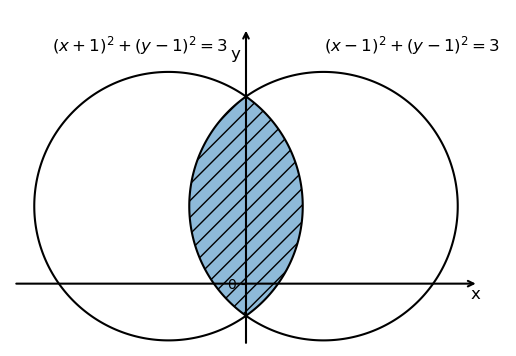
\includegraphics[width=0.9\columnwidth]{Img/cell1.png}
        \bicaption {解空间示意图。} {Solution Space Demo.}
        \label{fig:solution_space}
    \end{figure*}
    
    考虑逻辑公式$F = (x - 1)^2 + (y - 1)^2 \le 3 \wedge (x + 1)^2 + (y - 1)^2 \le 3$,构成的$R^2$空间图形如图\ref{fig:solution_space}所示。两个子句分别表示两个圆的内部,逻辑公式$F$表示同时存在两个圆内部的区域,即图中阴影区域。任何存在于阴影区域内的点都满足逻辑公式$F$,任何满足逻辑公式$F$的点都存在于阴影区域内。因此,解空间$S$是阴影区域的集合。
\label{ex:solution_space}
\end{example}
    
数学上,我们把这样的区域定义为胞腔。

\begin{definition}{\textbf{胞腔}}
对于$R^n$空间上的多项式集合$Q$,$Q$的一个胞腔(cell)是每个多项式$P \in Q$保持符号不变的$R^n$最大联通集合。对于任意的点$a \in R^n$,如果$a$在$Q$的胞腔内,则$a$满足$Q$中的所有多项式,我们记这个胞腔为$cell(Q, a)$。显然,胞腔是$R^n$空间的一个划分。
\end{definition}

对于逻辑公式而言,因为胞腔内的任意一点对每个多项式$P \in Q$保持符号不变,因此SMT公式对应的所有文字仍然保持布尔值不变,不会对SMT公示的满足或不满足造成任何影响。当找到其中任意一个满足逻辑公式的胞腔时,可以判定原公式可满足;当所有胞腔都被证明不可满足时,可以判定原公式不可满足。

给定逻辑公式,如何快速剔除不满足的胞腔并找到可满足的胞腔非常重要,因此现有的研究工作很多聚焦在更好地胞腔划分上。一般的胞腔划分是根据多项式的根和判别式等来判断的,从一个点得到胞腔的划分成为延拓。
\begin{definition}{\textbf{延拓}}
假定$R^n$上的多项式集合$Q$和点$a = (a_1, ..., a_n)$。给定一个变量$x_i (i = 1, 2,..., n)$,假定多项式$
\{q(a_1, ..., a_{i-1}, x_i, a_{i+1}, ..., a_n) | q(a_1, ..., a_{i-1}, x_i, a_{i+1}, ..., a_n) \nequiv 0, q \in Q\}$的实数根$r_1 < r_2 < \cdots < r_s$。一个点$a$关于变量$x_i$在集合$Q$上的延拓定义为一个满足如下性质的点集$\Lambda \subseteq R^n$:
\begin{itemize}
    \item 点$a \in \Lambda$并且对于$1 \leq j \leq s$均存在点$(a_1, ..., a_{i-1}, r_j, a_{i+1}, ..., a_n) \in \Lambda$。
    \item 对于任意点$b = (b_1, ..., b_n) \in \Lambda$,对于$j \in {1, ..., n} \\ {i}$有$b_j = a_j$。
    \item 对于任意的区间$I \in \{(-\infty, r_1), (r_1, r_2), \cdots, (r_{s-1}, r_s), (r_s, +\infty)\}$,都有唯一的$b = (b_1, ..., b_n) \in \Lambda$满足$b_i \in I$。
\end{itemize}
对于点集$\{a^{(1)}, ..., a^{(m)}\} \subseteq R^n$,定义集合关于变量$x_i$在$Q$上的延拓时$\bigcup_{j=1}^m \Lambda_j$,其中$\Lambda_j$是$a^{(j)}$关于变量$x_i$的延拓。
\end{definition}

\begin{example}
\begin{figure*}[]
    \centering
    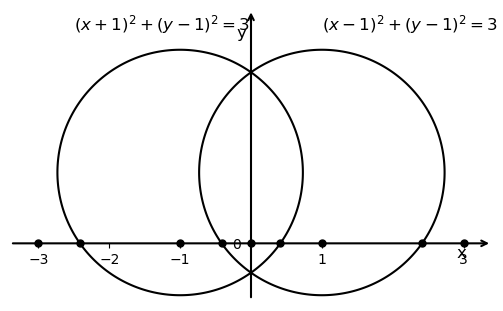
\includegraphics[width=0.45\columnwidth]{Img/cell2.png} \qquad
    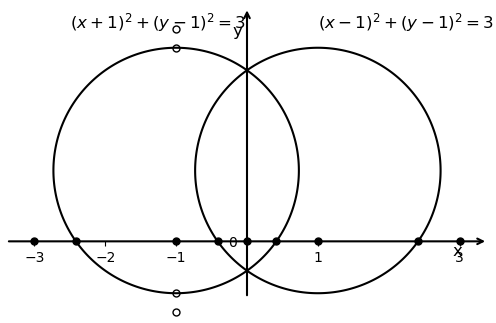
\includegraphics[width=0.45\columnwidth]{Img/cell3.png}
    \bicaption {延拓点集示意图。} {Expansion Demo.}
    \label{fig:expansion}
\end{figure*}
紧接着例子\ref{ex:solution_space},如图\ref{fig:expansion}所示,我们可以得到点$(0, 0)$关于$x$的延拓,即点集$\{(-3, 0), (-1-\sqrt{2}, 0), (-1, 0), (1-\sqrt{2}, 0), (0, 0), (\sqrt{2} - 1, 0), (1, 0), (1+\sqrt{2}, 0), (3, 0)\}$。这些点在$x$变量上分割了多项式的符号区间,从而划分了胞腔在$x$方向上的投影。右侧图的空心点构成了点$(-1, 0)$关于变量$y$的延拓,即点集$\{(-1, -1), (-1, 1-\sqrt{3}), (-1, 1+\sqrt{3}), (-1, 3)\}$,这些点在$y$方向上分开了多项式的符号区间,从而划分了胞腔在$y$方向上的投影。
\label{ex:expansion}
\end{example}
点$a$关于变量$x$的延拓点集事实上是点$a$在方向$x$上相邻胞腔的采样点,如何能够对$R^n$空间上的所有胞腔进行采样是我们接下来的话题。为此,我们引入柱形延拓的概念。

\begin{definition}{\textbf{柱形延拓}}
假设$R^n$上的多项式集合$Q$和点$a$。给定一个变量顺序$x_1 < x_2 < \cdots < x_n$,定义点$a$关于变量顺序在$Q$上的柱形延拓是$\bigcup_{i=1}^n \Lambda_i$,其中$\Lambda_1$是$a$关于变量$x_1$在$Q$上的延拓,并且$\Lambda_{i+1}$是$\Lambda_i$关于变量$x_{i+1}$在$Q$上的延拓。我们把最终的结果$\bigcup_{i=1}^n \Lambda_i$称为$Q$上的柱形延拓。
\end{definition}

柱形延拓可以理解为给定变量顺序下多维的点集延拓,其目的是在$R^n$空间的每一个胞腔上都有一个采样点。
\begin{figure*}[]
    \centering
    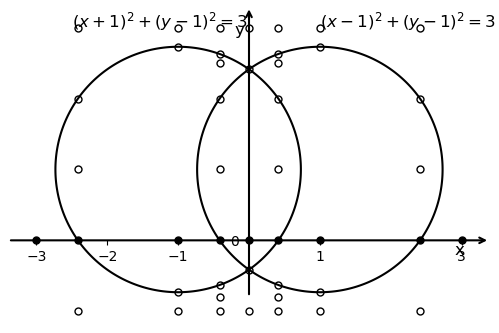
\includegraphics[width=0.9\columnwidth]{Img/cell4.png}
    \bicaption {柱形延拓示意图。} {Cylindrical Expansion Demo.}
    \label{fig:expansion2}
\end{figure*}
\begin{example}
\begin{table*}[]
    % \footnotesize
    \centering
    % \setlength{\tabcolsep}{0.4mm}% column separation
    % \renewcommand{\arraystretch}{1.2}%row space 
    \resizebox{\linewidth}{!}{
        \begin{tabular}{c | c | c | c}
            \hline
            点坐标 & $P_1: (x+1)^2 + (y-1)^2 = 3$根 & $P_2: (x -1)^2 + (y-1)^2 = 3$根 & 根集合\\\hline
            $x \mapsto -3$ & \emptyset & \emptyset & \emptyset \\\hline
            $x \mapsto -1-\sqrt{2}$ & \{0, 2\} & \emptyset & \{0, 2\} \\\hline
            $x \mapsto -1$ & $\{1 - \sqrt{3}, 1 + \sqrt{3}\}$ & \emptyset & $\{1 - \sqrt{3}, 1 + \sqrt{3}\}$ \\\hline
            $x \mapsto 1-\sqrt{2}$ & \{-0.63, 2.63\} & \{0, 2\} & \{-0.63, 0, 2, 2.63\} \\\hline
            $x \mapsto 0$ & $\{1 - \sqrt{2}, 1 + \sqrt{2}\}$ & $\{1 - \sqrt{2}, 1 + \sqrt{2}\}$ & $\{1 - \sqrt{2}, 1 + \sqrt{2}\}$ \\\hline
            $x \mapsto \sqrt{2} - 1$ & \{0, 2\} & \{-0.63, 2.63\} & \{-0.63, 0, 2, 2.63\} \\\hline
            $x \mapsto 1$ & \emptyset & $\{1 - \sqrt{3}, 1 + \sqrt{3}\}$ & $\{1 - \sqrt{3}, 1 + \sqrt{3}\}$ \\\hline
            $x \mapsto 1+\sqrt{2}$ & \emptyset & \{0, 2\} & \{0, 2\} \\\hline
            $x \mapsto 3$ & \emptyset & \emptyset & \emptyset \\\hline
        \end{tabular}
        }
        \bicaption{柱形延拓-区间计算。} {Demo of Computation of Cylindrical Expansion-Interval Splitting.}
\label{tab:expansion}
\end{table*}

\begin{table*}[]
    \tiny
    \centering
    \resizebox{0.65\linewidth}{!}{
        \begin{tabular}{c | c | c}
    \hline
    投影点 & 分割区间 & 延拓点集(采样点)\\\hline
    
    (-3, 0) & $(-\infty, \infty)$ & (-3, 0)\\\hline
    
    \multirow{5}{*}{$(-1-\sqrt{2}, 0)$} & $(-\infty, 0)$ & $(-1-\sqrt{2}, -1)$ \\ & [0, 0] & $(-1-\sqrt{2}, 0)$ \\ & (0, 2) & $(-1-\sqrt{2}, 1)$ \\ & [2, 2] & $(-1-\sqrt{2}, 2)$ \\ & (2, \infty) & $(-1-\sqrt{2}, 3)$ \\\hline
    
    \multirow{5}{*}{(-1, 0)} & $(-\infty, 1-\sqrt{3})$ & (-1, -1) \\
    & $[1-\sqrt{3}, 1-\sqrt{3}]$ & $(-1, 1-\sqrt{3})$ \\
    & $(1-\sqrt{3}, 1+\sqrt{3})$ & (-1, 0) \\
    & $[1+\sqrt{3}, 1+\sqrt{3}]$ & $(-1, 1+\sqrt{3})$ \\
    & $(1+\sqrt{3}, \infty)$ & (-1, 3) \\\hline

    \multirow{9}{*}{$(1-\sqrt{2}, 0)$} & $(-\infty, -0.63)$ & $(1-\sqrt{2}, -1)$ \\
    & [-0.63, -0.63] & $(1-\sqrt{2}, -0.63)$ \\
    & (-0.63, 0) & $(1-\sqrt{2}, -0.5)$ \\
    & [0, 0] & $(1-\sqrt{2}, 0)$ \\
    & (0, 2) & $(1-\sqrt{2}, 1)$ \\
    & [2, 2] & $(1-\sqrt{2}, 2)$ \\
    & (2, 2.63) & $(1-\sqrt{2}, 2.5)$ \\
    & [2.63, 2.63] & $(1-\sqrt{2}, 2.63)$ \\
    & (2.63, \infty) & $(1-\sqrt{2}, 3)$ \\\hline

    \multirow{5}{*}{(0, 0)} & $(-\infty, 1-\sqrt{2})$ & $(0, -1)$ \\
    & $[1-\sqrt{2}, 1-\sqrt{2}]$ & $(0, 1-\sqrt{2})$ \\
    & $(1-\sqrt{2}, 1+\sqrt{2})$ & (0, 0) \\
    & $[1+\sqrt{2}, 1+\sqrt{2}]$ & $(0, 1+\sqrt{2})$ \\
    & $(1+\sqrt{2}, \infty)$ & (0, 3) \\\hline

    \multirow{9}{*}{$(\sqrt{2}-1, 0)$} & $(-\infty, -0.63)$ & $(\sqrt{2}-1, -1)$ \\
    & [-0.63, -0.63] & $(\sqrt{2}-1, -0.63)$ \\
    & (-0.63, 0) & $(\sqrt{2}-1, -0.5)$ \\
    & [0, 0] & $(\sqrt{2}-1, 0)$ \\
    & (0, 2) & $(\sqrt{2}-1, 1)$ \\
    & [2, 2] & $(\sqrt{2}-1, 2)$ \\
    & (2, 2.63) & $(\sqrt{2}-1, 2.5)$ \\
    & [2.63, 2.63] & $(\sqrt{2}-1, 2.63)$ \\
    & (2.63, \infty) & $(\sqrt{2}-1, 3)$ \\\hline

    \multirow{5}{*}{(1, 0)} & $(-\infty, 1-\sqrt{3})$ & $(1, -1)$ \\
    & $[1-\sqrt{3}, 1-\sqrt{3}]$ & $(1, 1-\sqrt{3})$ \\
    & $(1-\sqrt{3}, 1+\sqrt{3})$ & (1, 0) \\
    & $[1+\sqrt{3}, 1+\sqrt{3}]$ & $(1, 1+\sqrt{3})$ \\
    & $(1+\sqrt{3}, \infty)$ & (1, 3) \\\hline

    \multirow{5}{*}{$(1+\sqrt{2}, 0)$} & $(-\infty, 0)$ & $(1+\sqrt{2}, -1)$ \\
    & [0, 0] & $(1+\sqrt{2}, 0)$ \\
    & (0, 2) & $(1+\sqrt{2}, 1)$ \\
    & [2, 2] & $(1+\sqrt{2}, 2)$ \\
    & (2, \infty) & $(1+\sqrt{2}, 3)$ \\\hline

    (3, 0) & $(-\infty, \infty)$ & (3, 0) \\\hline
\end{tabular}
        }
        \bicaption{柱形延拓-采样点生成。} {Demo of Computation of Cylindrical Expansion-Sampling Points.}
\label{tab:expansion2}
\end{table*}

紧接着例子\ref{ex:expansion},如图\ref{fig:expansion2}所示,图中所有的实心点和空心点共同构成了基于变量顺序$x < y$的多项式$Q$的柱形延拓,达到了每个胞腔上均有一个采样点的效果。具体的步骤是,首先点$(0, 0)$关于变量$x$形成延拓(实心点),然后每一个实心点关于变量$y$各自形成延拓(空心点),最终所有点的集合共同构成了柱形延拓。表格\ref{tab:expansion}展示了在实心点处根据多项式集合的根分割得到的区间。表格\ref{tab:expansion2}展示了在每一个分割区间进行采样得到的结果,即最终的柱形延拓点集(空心点)。
\end{example}

\begin{definition}{\textbf{柱形完备}}
对于$R^n$上的多项式集合$Q$,给定一个变量顺序$x_1 < x_2 < \cdots < x_n$,称$Q$对于变量顺序是柱形完备的,当任意的点$a \in R^n$和其关于$Q$的柱形延拓$\Lambda$,$Q$的每一个胞腔都包含至少一个$\Lambda$的点。
\end{definition}
具体的证明请参阅\cite{Caviness2004QuantifierEA,Collins74}。

\subsection{量词消去与柱形代数分解}
根据前文的讨论,我们引出基于多项式解空间的一种量词消去算法-柱形代数分解(Cylindarical Algebraic Decomposition)。

\begin{definition}{\textbf{量词消去}}
量词消去指的是给定一个带有量词的逻辑公式$\varphi$,找到另一个不带有两次的逻辑公式$\psi$,使得$\varphi$和$\psi$的逻辑等价,记为$\varphi \Leftrightarrow \psi$。量词消去的目的是将逻辑公式转化为更易处理的形式,以更好地判断问题的可满足性。
\end{definition}

\begin{example}
考虑多项式$P_s(x, y) = s(x^2 + y^2 - 1) + (1 - s)(xy - 1)$,和逻辑公式$\varphi = \exists R \forall x, y [P_s(x, y) = 0 \Rightarrow x^2 + y^2 \leq R^2]$。量词消去即求解当$s$取什么值的时候逻辑公式$\varphi$满足。通过量词消去工具,我们可以得到$\varphi \Leftrightarrow s \le -1 \wedge s > \frac{1}{3}$。\label{ex:quantifier_elimination}
\end{example}

多项式理论常用的一种量词消去是柱形代数分解(Cylindarical Algebraic Decomposition, CAD)。其核心仍然是把$R^n$空间划分成多个符号一致的胞腔,然后通过判断每个胞腔是否满足逻辑公式进而得到给定变量的赋值区间。如图\ref{fig:CAD}所示,给定变量顺序和多项式集合,柱形代数分解可以分为三个步骤:投影、实根隔离和提升,具体的步骤如下:
\begin{itemize}
    \item \textbf{投影(projection):}从多项式集合开始,每次消去一个变量,生成新的多项式集合,新多项式继续消去变量直到只剩下一个变量为止,记为$proj(P)$。
    \item \textbf{实根隔离(root isolation):}当投影只剩下一个变量时,对当前多项式集合求所有根,得到顺序排列的一组根,这些根表示了胞腔在当前变量上的分割。
    \item \textbf{提升(lift):}提升是对投影阶段得到的多项式集合进行采样。投影从单变量多项式开始,从采样点继续对上一个投影多项式进行采样,直到最终对$R^n$多项式采样,最终保证了每个胞腔得到了采样点。
\end{itemize}

\begin{figure*}[t]
    \centering
    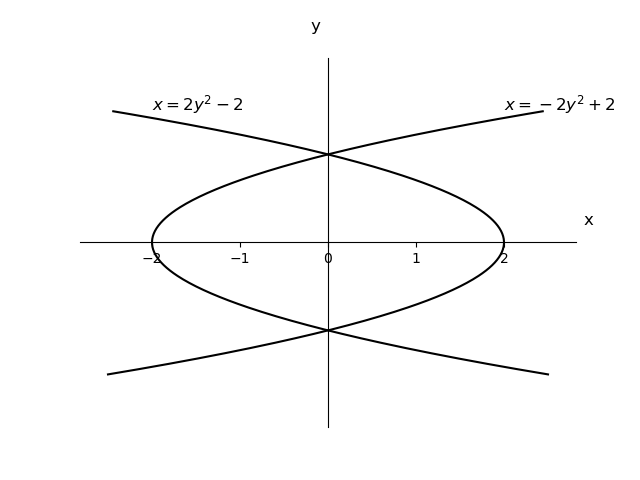
\includegraphics[width=\columnwidth]{Img/cad.png}
    \bicaption {柱形代数分解步骤示意图。} {Demo of Cylindarical Algebraic Decomposition Steps.}
\label{fig:CAD}
\end{figure*}
投影算子(projection operator)指的是投影过程中对多项式集合的计算,比如Collins算子\cite{Collins74}和McCallum算子\cite{McCallum98}。后者因为其计算相对便捷,被广泛应用于量词消去工具和SMT求解器中。

McCallum算子用到的计算包括结式、判别式和求根等操作。
\begin{definition}{\textbf{结式(resultant)}}
对于两个多项式$P_1, P_2 \in R[x_1, ..., x_n]$,假定$$
P_1 = a_m x_n^{d_m} + a_{m-1} x_n^{d_{m-1}} + \cdots + a_0,
$$
$$
P_2 = b_n x_n^{e_n} + b_{n-1} x_n^{e_{n-1}} + \cdots + b_0.
$$
定义$P_1$和$P_2$的结式$Res(P_1, P_2, x_n)$为:
$$
Res(P_1, P_2, x_n) = 
\begin{vmatrix}
    a_m & a_{m-1} & \cdots & a_0 \\
    & a_m & a_{m-1} & \cdots & a_0 \\
    & \ddots & \ddots & \ddots & \ddots & \\
    & & a_m & a_{m-1} & \cdots & a_0 \\

    b_n & b_{n-1} & \cdots & b_0 \\
    & b_n & b_{n-1} & \cdots & b_0 \\
    & \ddots & \ddots & \ddots & \ddots & \\
    & & b_n & b_{n-1} & \cdots & b_0 \\
    \end{vmatrix}
$$
\end{definition}

\begin{definition}{\textbf{判别式(discreminant)}}

对于多项式$P \in R[x_1, ..., x_n]$,假定$$
P = a_m x_n^{d_m} + a_{m-1} x_n^{d_{m-1}} + \cdots + a_0.
$$
定义$P$关于变量$x_n$的判别式$Disc(P, x_n)$为:  
$$
Disc(P, x_n) = \frac{(-1)^{\frac{m(m-1)}{2}}}{a_m} Res(f, \frac{\partial f}{\partial x_n}, x_n). 
$$
\end{definition}

\begin{definition}{\textbf{McCallum投影算子(McCallum Projection Operator)}}

假定$F = \{f_1, f_2, \dots, f_m\}$ 是一组$R^n$上的多项式。McCallum投影算子$proj(F, x_i)$是从$F$到$R^{n-1}$上的多项式集合$proj_m(F)$的一组映射,包含以下元素:
\begin{itemize}
    \item $F$中每个多项式的系数
    \item $F$中每个多项式关于变量$x_n$的判别式
    \item $F$中每两个不同多项式$f_i, f_j$关于变量$x_n$的结式
\end{itemize}
实际计算中,多项式集合的元素通过因式分解化为最简系数的形式,对结果不产生影响。
\end{definition}

\begin{example}
我们给出CAD算法的一个例子。假设$F = \{P_1: x - 2y^2 + 2, P_2: x + 2y^2 - 2\}$,我们规定变量顺序为$y < x$,按步骤计算如下:
\begin{enumerate}
    \item \textbf{投影}:计算对于变量$y$的投影$proj(F, y)$
    \begin{itemize}
        \item 化简后系数多项式为$\{x + 2, x - 2\}$
        \item 化简后判别式为$\{x + 2, x - 2\}$
        \item 化简后结式为$\{x\}$。
    \end{itemize}
    得到投影多项式$proj(F, y) = \{x, x - 2, x + 2\}$

    \item \textbf{实根隔离}:我们对$proj(F, y)$的每个多项式求根,得到根集合$\{-2, 0, 2\}$。
    \item \textbf{提升}:我们对根集合分得的区间进行提升,进一步采样所有胞腔,结果如表格\ref{tab:cad}所示。
    \begin{table*}[]
        \tiny
        \centering
        \resizebox{0.65\linewidth}{!}{
            \begin{tabular}{c | c | c | c | c}
            \hline
            分割区间 & $x$采样点 & $y$根集合 & $(x, y)$采样点 & 符号($P_1, P_2$)\\\hline
            \multirow{5}{*}{$(-\infty, -2)$} & \multirow{5}{*}{$x \rightarrow -3$} & \multirow{5}{*}{$\{-\frac{\sqrt{10}}{2}, \frac{\sqrt{10}}{2}\}$} & (-3, 2) &  (-, +)\\
            & & & $(-3, \frac{\sqrt{10}}{2})$ & (-, 0)\\
            & & & $(-3, 0)$ & (-, -)\\
            & & & $(-3, -\frac{\sqrt{10}}{2})$ & (-, 0)\\
            & & & $(-3, -2)$ & (-, +)\\\hline

            \multirow{7}{*}{$[-2, -2]$} & \multirow{7}{*}{$x \rightarrow -2$} & \multirow{7}{*}{$\{0. -\sqrt{2}, \sqrt{2}\}$} & (-2, 2) &  (-, +)\\
            & & & $(-2, \sqrt{2})$ & (-, 0)\\
            & & & (-2, 1) & (-, -)\\
            & & & (-2, 0) & (0, -)\\
            & & & (-2, -1) & (-, -)\\
            & & & $(-2, -\sqrt{2})$ & (-, 0)\\
            & & & (-2, -2) & (-, +)\\\hline
            \end{tabular}

            To be Done
        }
        \bicaption{柱形代数分解-提升。} {Demo of Cylindrical Algebraic Decomposition - Lift.}
        \label{tab:cad}
    \end{table*}
\end{enumerate}
\label{ex:cad}    
\end{example}

\section{非线性实数理论求解现状}
\subsection{CDCL(T)算法}
CDCL(T) (Conflict Driven Clause Learning for Theories)算法主要是在SAT问题的CDCL搜索框架上增加了理论求解器(Theory Solver),主要的搜索思路包括单元传播、分支决策、冲突分析及回退等CDCL常见技术。理论求解器的作用是对给定的布尔骨架赋值进行推理,当全部布尔骨架得到赋值时通过理论分析返回问题可满足或者报告冲突。具体框架请参见图\ref{fig:cdclt}。

非线性实数的理论求解器主要目的是判断多项式不等式集合的一致性,主要方法可以分为以下几种:
\begin{itemize}
    \item \textbf{区间约束传播(interval constraint propagation, ICP):} 通过变量或者单项式的赋值区间推导出多项式的赋值区间,根据这些区间快速判断一些常见的不一致性。
    \item \textbf{虚拟替代(virtual substitution, VS):} 通过替换多项式中的变量,将多项式转化为更简单的形式,进而判断问题的可满足性。
    \item \textbf{柱形代数分解(cylindrical algebraic decomposition, CAD):} 如前文所述,通过把$R^n$空间划分为多个符号一致的胞腔,逐一排查的方式来推出问题的可满足性。
    \item \textbf{增量线性化(incremental linearization):}把一些多项式线性化,然后使用线性求解器检测问题可满足性,一般是不完备的。
\end{itemize}

\begin{figure*}[t]
    \centering
    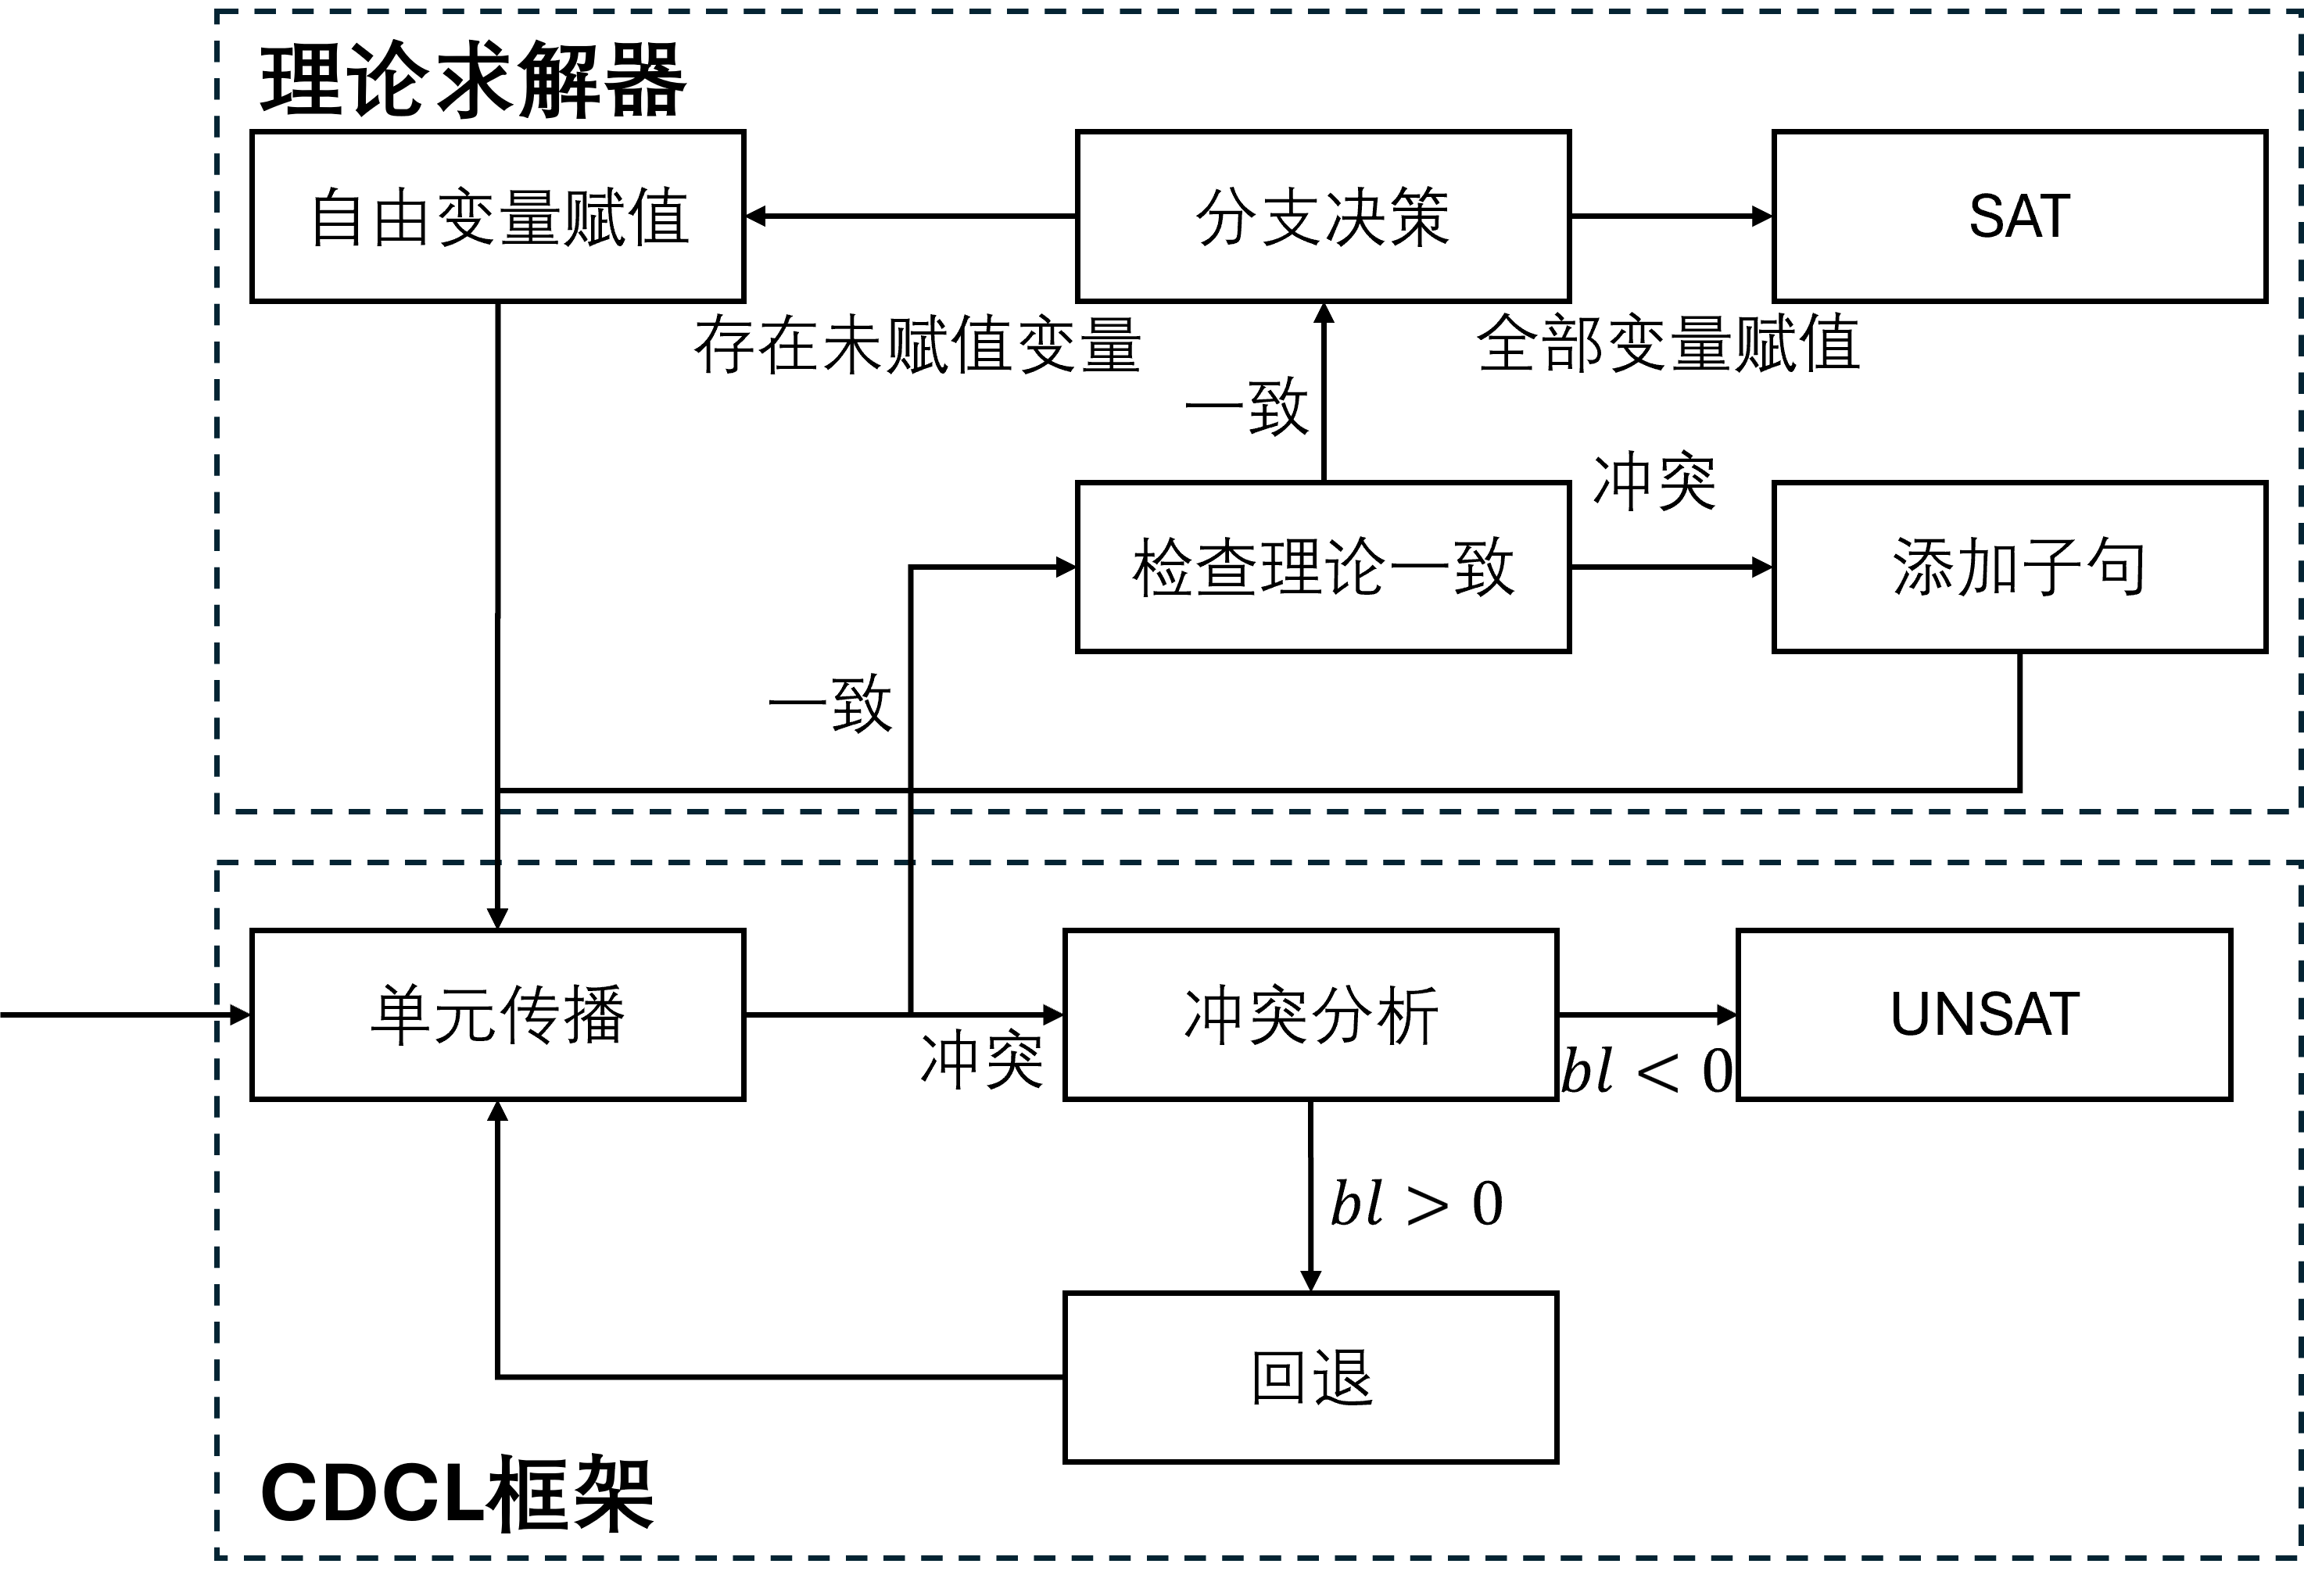
\includegraphics[width=\columnwidth]{Img/cdcl_t.png}
    \bicaption {CDCL(T)框架示意图。} {Demo of CDCL(T) Framework.}
    \label{fig:cdclt}
\end{figure*}

\subsection{MCSAT/NLSAT方法}
MCSAT(Model-Constructing Satisfiability)和NLSAT(NonLinear Satisfiability)是另一种具有CDCL结构的算法,核心的思想仍然是决策赋值、冲突分析和回退。与CDCL(T)不同的是,MCSAT/NLSAT算法加入了基于可行域的算术变量推理,允许在脱离布尔骨架的情况下直接对算术变量进行赋值,一些基本概念介绍如下:
\begin{itemize}
    \item \textbf{决策层数(level):}指文字层面的决策层数,包括布尔文字和算术文字。
    \item \textbf{决策阶段(stage):}指算术变量赋值次数。
    \item \textbf{日志(trace):}一种记录算法更新的线性结构,包括可行域的更新、决策变量的赋值等。
    \item \textbf{算术传播(arithmetic propagation):}基于可行域的文字层面的传播,可以直接推断某些文字的可满足性。
\end{itemize}
其中,MCSAT/NLSAT最关键的步骤就是根据当前变量和文字的可行域关系进行算术文字赋值,假设算术变量的可行域是$curr\_set$,文字的可行域是$lit\_set$,算术传播分为以下几种情况:
\begin{itemize}
    \item \textbf{$lit\_set = \emptyset$:}任何赋值都不能使文字满足,判断文字为$\bot$。比如当$x \mapsto -1$时,文字$y^2 \leq x$不可满足。
    \item \textbf{$lit\_set = R$:}任何赋值都可以使文字满足,直接赋值文字为$\top$。比如文字$x^2 \geq -1$一定满足。
    \item \textbf{$curr\_set \subseteq lit\_set$:}当前文字的可行域包括了算术变量的可行域,因此可以直接判断文字满足。比如当$x \in [-2, 2]$时,文字$x^2 \leq 10$一定满足。
    \item \textbf{$curr\_set \cap lit\_set = \emptyset$:}任何可行域内的赋值都不会让文字满足,因此直接赋值文字为$\bot$。比如当$x \in [-2, 2]$时,文字$x^2 \geq 10$不可满足。
\end{itemize}

例\ref{ex:nlsat}给出了一个MCSAT/NLSAT搜索的具体例子。

\begin{example}
考虑公式$F=(P_1: (x-2)^2 + y^2 \le 4) \wedge (P_2: x - y \ge 0)$。假设我们的搜索顺序是$x < y$,算法的搜索过程如下:
\begin{enumerate}
    \item \textbf{决策算术变量:}赋值$x \mapsto 5$。
    \item \textbf{可行域计算:}计算$P_1$关于变量$y$的可行域是$\emptyset$,发现冲突。
    \item \textbf{冲突分析:}对公式$\exists y. (x-2)^2 + y^2 \le 4$进行量词消去,通过柱形代数分解得到实根$\{0, 4\}$,生成新的学习子句$x \le 4$。
    \item \textbf{回退:}回退到x未赋值的状态。
    \item \textbf{决策算术变量:}重新赋值$x \mapsto 2$。
    \item \textbf{可行域计算:}计算$P_1$关于变量$y$的可行域是$[-2, 2]$,$P_2$关于变量$y$的可行域是$(-\infty, 2]$,取交集得到可行域是$[-2, 2]$。
    \item \textbf{决策算术变量:}赋值$y \mapsto 0$。所有变量得到赋值,返回SAT。
\end{enumerate}
\label{ex:nlsat}
\end{example}

\subsection{局部搜索算法}


\subsection{其他方法}


\section{约束满足问题求解现状}

首先,本文先介绍CSP的定义,它的特点是要求变量的值域有限且离散。前置概念的定义如下。

对于一个变量 $x$,本文用 $D(x)$ 来表示 $x$ 的域,即可以赋予 $x$ 的一组可能的值。通常,使用简写 $x \in \{d_1, \dots, d_m\}$ 来定义 $D(x) = \{d_1, \dots, d_m\}$。特别地,在本文的讨论中仅考虑那些具有有限域的变量。

设 $Y = y_1, y_2, \dots, y_k$ 是一组有限的变量序列,其中 $k > 0$。一个关于 $Y$ 的约束 $c \in C$ 是变量序列 $Y$ 中变量的域的笛卡尔积的子集,即 $c \subseteq D(y_1) \times D(y_2) \times \cdots \times D(y_k)$。约束可以写作 $c(Y)$ 或 $c(y_1, y_2, \dots, y_k)$。如果约束定义在两个变量上,称之为\textit{二元约束}。如果约束定义在两个以上的变量上,称之为\textit{全局约束}。

\begin{definition}[\textbf{约束满足问题}]
    一个CSP,由一组有限的变量序列 $X = x_1, x_2, . . . , x_n$ 及其各自的域 $D = D(x_1), D(x_2), \dots, D(x_n)$ 组成,同时伴有一组约束 $C$,每个约束都在 $X$ 的一个子序列上。为了简化表示,在表示特定的约束集合时经常省略大括号“\{\}”,从而一个CSP被表示为 $P = (X, D, C)$。
\end{definition}

之后,本文给出CSP解的定义。设 $P = (X, D, C)$ 为一个 CSP,其中 $X = x_1, x_2, \dots, x_n$ 且 $D = D(x_1), D(x_2), \dots, D(x_n)$。如果元组 $(d_1, \dots, d_n) \in D(x_1) \times \cdots \times D(x_n)$,并且 $(d_{i_1}, d_{i_2}, \dots, d_{i_m}) \in c$,其中$c \in C$,那么,称关于 $X$ 的这组赋值满足在变量 $x_{i_1}, x_{i_2}, \dots, x_{i_m}$ 上的约束 $C$。

对于变量序列 $K$,定义 $D(K) = \bigcup_{x \in K} D(x)$。当变量 $x$ 的域 $D(x)$ 是单元素集,即 $D(x) = \{d\}$ 时,将其简写为 $x = d$,记作\textit{单域}。

一个CSP是\textit{一致的},如果这个CSP存在解。相反,不存在解的CSP是\textit{不一致的}。一个\textit{失败的}CSP指具有空域(也即存在变量的值域为空)的CSP,或者只有单域的CSP且这些值并不能共同构成CSP的解。一个CSP是\textit{已解决的},若该CSP只有单域,并且其中的赋值可以共同构成CSP的解。需要注意的是,一个失败的CSP也是不一致的,但并非所有不一致的CSP都是失败的。

设 $P = (X, D, C)$ 和 $P' = (X , D', C')$ 都是 CSP。如果 $P$ 和 $P'$ 有相同的解集,那么它们被称为\textit{等价的}。如果 $P$ 和 $P'$ 等价,且对所有的 $x \in X$,都有 $D(x) \subseteq D'(x)$,那么 $P$ 小于 $P'$。这种关系记作 $P \preceq P'$。如果 $P \preceq P'$ 并且至少存在一个 $x \in X$ 使得 $D(x) \subset D'(x)$,那么 $P$ 严格小于 $P'$。这种关系记作 $P \prec P'$。当 $P \preceq P'$ 和 $P' \preceq P$ 都成立时,记作 $P \equiv P'$。

\subsection{约束规划求解}

约束规划的目标是寻找给定的CSP的一个解(或所有解)。求解过程中,值域过滤、约束传播和搜索是交织进行的。

对CSP的解(或所有解)的寻找是通过迭代地将一个CSP分解为更小的CSP来进行的。这个分解过程被称为\textit{构建搜索树}。树的一个节点代表一个CSP。最初,在根节点,得到一个待解决的CSP,记作$P_0$。如果$P_0$既没有被解决也没有失败,就将$P_0$分解为两个或更多的CSP,记作$P_1$,$P_2$,…,$P_k$($k>1$)。同时,必须确保$P_0$的所有解都被保留,而且没有多余的解被添加到$P_0$中。从而,$P_1$,$P_2$,…,$P_k$的解集的并集等于$P_0$的解集。此外,每个CSP $P_i$($i>0$)应该严格小于$P_0$,以确保分解过程能够终止。接下来,会根据上述相同的标准分解每个CSP $P_1$,$P_2$,…,$P_k$。分解会一直进行,直到所有CSP被分解为失败的或已解决的CSP。失败和已解决的CSP是搜索树的叶子节点。

搜索树的大小与$P_0$中变量数量呈指数关系。为了减小搜索树的大小,约束规划使用了一个叫做\textit{约束传播}的过程。给定一个约束$C$,一个\textit{值域过滤算法}会从$C$中的变量的值域中移除与$C$不一致的值。算法必须保留所有的解并且不向$C$中添加任何解。每当一个不一致的值域值被移除,其效果会通过所有其他共享相同对应变量的约束进行传播。这个迭代过程持续进行,直到在CSP中的所有约束都未检测到更多的不一致值。此时,可以称CSP是\textit{局部一致的}。局部一致性反映了算法并没有得到一个全局一致的CSP,而是得到了一个所有约束都是局部的,也即单独的、一致的CSP。这里本文将介绍四个常见的局部一致性:\textit{弧一致性}、\textit{超弧一致性}、\textit{边界一致性}和\textit{区间一致性}。

\begin{definition}[\textbf{弧一致性}]
    一个二元约束$c(x_1, x_2)$是弧一致的,如果对于$x_1$的所有值$d_1 \in D(x_1)$,存在一个值$d_2 \in D(x_2)$使得$(d_1, d_2) \in c$,并且对于$x_2$的所有值$d_2 \in D(x_2)$,存在一个值$d_1 \in D(x_1)$使得$(d_1, d_2) \in c$。
\end{definition}

\begin{definition}[\textbf{超弧一致性}]
    一个约束$c(x_1, ..., x_m)$($m>1$)是超弧一致的,如果对于所有$i \in \{1, ..., m\}$和所有$d_i \in D(x_i)$,存在值$d_j \in D(x_j)$(其中$j \in \{1, ..., m\} - i$),使得$(d_1, ..., d_m) \in c$。
\end{definition}

超弧一致性又称\textit{全局弧一致性}(Generalized Arc Consistency,GAC),相较于弧一致性限制性更强,应用也更广。需要注意的是,弧一致性相当于应用于二元约束的超弧一致性。弧一致性和超弧一致性都确保每个域中的所有值都属于满足约束的元组,与当前变量域相关。另外两种局部一致性概念主要关注变量域的边界。因此,当应用这些定义时,假设涉及的变量域是一个固定的、线性有序的、有限域的元素集的子集。设$D$是这样的一个域,定义$min D$和$max D$分别为其最小值和最大值。此外,使用大括号“\{ \}”和方括号“[ ]”来分别表示一组域值和一个域值区间。

\begin{definition}[\textbf{边界一致性}]
    一个约束$c(x_1, ..., x_m)$($m>1$)是边界一致的,如果对于所有$i \in \{1, ..., m\}$和每个值$d_i \in \{min D(x_i), max D(x_i)\}$,存在值$d_j \in [min D(x_j), \\ max D(x_j)]$(其中$j \in \{1, ..., m\} - i$),使得$(d_1, ..., d_m) \in c$。
\end{definition}

\begin{definition}[\textbf{区间一致性}]
    一个约束$c(x_1, ..., x_m)$($m>1$)是区间一致的,如果对于所有$i \in \{1, ..., m\}$和所有$d_i \in D(x_i)$,存在值$d_j \in [min D(x_j), max D(x_j)]$(其中$j \in \{1, ..., m\} - i$),使得$(d_1, ..., d_m) \in c$。
\end{definition}

在分解一个CSP之后,值域过滤和约束传播被应用到更小的CSP上。值的移除导致搜索树变小,从而加速了解决过程。同时,花费在约束传播上的时间应该小于它引发的加速,以便改善效果显著。关于约束传播过程的详细描述可以在\cite{apt1999essence}和\cite{apt2003principles}中找到,这里不再展开。总之,本文希望应用高效的过滤算法,其效率通常由应用于约束的局部一致性的概念来决定,而在解决过程中何时应用哪种局部一致性的概念则取决于问题本身。

当前主流的求解器分为完备的和启发式的求解器,一些求解器是商用的,而一些则是开源的,他们具有不同的特点,本文介绍三个主流的CP求解器。

\begin{itemize}
% \renewcommand{\labelenumi}{\theenumi)}
    \item Choco。Choco\footnote{\href{https://choco-solver.org/}{https://choco-solver.org/}}是一个基于Java的约束满足问题(CSP)求解库。它提供了一种声明式语言,用于描述和解决各种复杂的约束满足问题。Choco常被用作研究和教学工具,并且支持各种类型的约束,包括数值约束、逻辑约束等。
    \item CPLEX Optimizer。CPLEX Optimizer\footnote{\href{https://www.ibm.com/products/ilog-cplex-optimization-studio}{https://www.ibm.com/products/ilog-cplex-optimization-studio}}是IBM ILOG的一款产品,它包含一个称为CP Optimizer的模块,这是一个约束规划求解器。其主要优点是拥有丰富的API,支持多种编程语言,如C++、Java、Python等,并且它的求解速度非常快,可以处理非常大规模的问题。
    \item Yuck。Yuck是一个基于Scala的运筹学和约束规划库,它的主要特点是它采用了一种基于邻域搜索的算法,可以在解空间中快速找到优质的解。作为一款启发式求解器,他在近几年的CP求解启发式赛道中都是第一名。
\end{itemize}

这些求解器都支持集成在Minizinc\cite{nethercote2007minizinc}中。MiniZinc是一种中间级别的约束建模语言,设计用于描述各种组合优化问题。它的主要目标是提供一种简单、可移植且高效的方式来描述这些问题,以便可以使用各种不同的求解器来解决它们。并且,它支持数组、集合和函数等高级数据结构,以及各种数学和逻辑运算符,并且可以使用CPLEX、Choco、Gecode等求解器作为后端求解器,这使得用户可以在不改变模型的情况下尝试不同的求解器和算法。

\subsection{其他求解方法}

除了CP求解器外,有许多其他的求解技术也可以用来处理CSP,它们来自于不同的研究领域。其中,\textit{布尔可满足性(SAT)求解器}、\textit{可满足性模理论(SMT)求解器}和\textit{整数线性规划(ILP)求解器}是最常用的三种。接下来,本文将介绍这三种求解技术,以及它们在处理CSP时的优势和应用情景。

逻辑公式可满足性问题要求判定一个逻辑公式是否存在使得公式为真的赋值,SAT和SMT问题是其中最主要的两个可满足性问题。SAT问题是第一个被证明为NP完全的问题,是计算机科学的核心问题,也是数理逻辑的基础问题。然而,SAT问题的表达能力和应用范围有其局限性。许多现实问题牵涉到各种领域知识,这就需要用表达能力更强的逻辑公式,比如一阶逻辑公式。尽管一阶逻辑语言是不可判定的,但许多应用只需处理一些背景理论来解释特定的谓词和函数记号的一阶逻辑公式。这类公式被称为SMT公式,它对SAT问题进行了扩展,将其中的布尔变量用背景理论谓词取代。常见的SAT求解器有MiniSAT、Kissat等,而主流的SMT求解器则包含Z3、CVC5等。

\begin{definition}[\textbf{布尔可满足性}]
    一个SAT问题由一系列的布尔变量和逻辑运算符(如与、或、非)构成,对该问题的求解涉及到查找一个给定的布尔公式的满足赋值,使得整个公式的结果为真。
\end{definition}

\begin{definition}[\textbf{可满足性模理论}]
    一个SMT问题可以表示为一个三元组,包含变量集合(可以是整数、实数或者字符串)、函数符号集合(比如常见的运算符、量词等操作)、以及由变量和函数组成的约束集合。
    对该问题的求解涉及到一组变量的赋值,使得约束集合中的约束全部可满足。
\end{definition}

SAT问题是NP完全问题,但现代的SAT求解器已经能够处理数百万个变量和数千万个约束的问题。
将CSP转化为SAT问题的关键步骤是将CSP的变量和约束转化为布尔变量和布尔公式。具体来说,对于CSP中的每一个变量和它的每一个可能的值,都定义一个对应的布尔变量。如果CSP变量被赋予该值,则对应的布尔变量为真;否则为假。然后,可以使用“at most one”和“at least one”的编码方式来保证CSP中的每个变量只能取一个值。同时,CSP的其他约束也可以通过定义相应的布尔公式来实现。

将CSP编码为SMT问题的过程相对直接。由于SMT支持整数变量和约束,以及各种数学函数,因此可以直接将CSP中的变量、约束和函数映射到SMT问题中。
这样,CSP就可以被转化为一个等价的SAT/SMT问题,进而利用相应求解器求解。一般来言,在编码CSP时,SAT的编码复杂度要高很多,但比涉及高阶逻辑的SMT求解器拥有更好的性能。

最后是ILP,它是线性规划(LP)的一种扩展。线性规划问题包含一组线性约束条件和一个线性目标函数,问题的目标是在满足这些约束条件的前提下,找到使目标函数取得最大(或最小)值的变量的取值,而ILP则要求所有的决策变量都是整数。
由于CSP中的变量通常也是整数,因此CSP可以很自然地映射为ILP问题。常见的ILP求解器有Gurobi、SCIP等。

这些算法为解决CSP提供了新的视角,尽管某些转换可能相对复杂,可能会影响性能或效率,但它们也弥补了CP求解器在特定问题时的不足。

\section{AllDifferent约束求解现状}

由于目前AllDifferent约束的过滤算法及后续算法都要用到图论的相关知识,所以本文先介绍图论以及相关的最大匹配算法,之后介绍AllDifferent约束的过滤算法以及基于该算法的一些改进策略。

\subsection{图论基础}

本文用$G = (V, E)$表示一个(无向)图,其中$V$是一个有限的顶点集,而$E$是来自$V$的无序对的多重集,称为边。顶点$u \in V$和$v \in V$之间的边记作$uv$。
如果存在一个分区$S, T$,使得$E \subseteq \{st | s \in S, t \in T \}$,那么图$G = (V, E)$称为\textit{二部图},写作$G = (S, T, E)$。

在图$G = (V, E)$中,\textit{游走}指一个序列$P = v_0, e_1, v_1, \dots, e_k, v_k$,其中$k \geq 0$,$v_0, v_1, \dots, v_k \in V$,$e_1, e_2, \dots, e_k \in E$,并且对于$i = 1, \dots, k$,有$e_i = v_{i-1}v_i$。如果$v_0, \dots, v_k$是不同的,那么这个游走就被称为一条\textit{路径}。一个闭合的路径,即$v_0 = v_k$,称为\textit{回路}。

图$G = (V, E)$的子图是一个图$G' = (V', E')$,它满足$V' \subseteq V$和$E' \subseteq \{uv | u \in V', v \in V', uv \in E\}$。称子图$G' = (V', E')$为图$G = (V, E)$的\textit{最大连通子图},若对于$V'$中的每一对$u, v$,在$G'$中都存在一条$u$到$v$的路径。

有向图是一个对$G = (V, A)$,其中$V$是一个有限的顶点集,$A$是来自$V$的有序对的多重集,称为弧,从$u \in V$到$v \in V$的弧记作$(u, v)$。
类似于无向二部图,如果存在一个分区$S, T$,使得$A \subseteq \{(s, t) | s \in S, t \in T \}$,那么有向图$G = (V, A)$就是二部图。也写作$G = (S, T, A)$。
此外,关于有向图的路径、回路、子图、最大连通子图等概念和无向图类似,这里不再展开。

在有向图中,如果存在两个顶点$s$和$t$,从$s$可以通过一条有向路径到达$t$,同时也可以从$t$通过一条有向路径到达$s$,那么就说两个顶点\textit{相互到达}。如果在一个有向图中,存在一个顶点集$V$,对于集合中的任意两个顶点$u$和$v$都可以相互到达,称$V$为\textit{强连通分量}(Strongly Connected Component,SCC)。

图$G = (V, E)$的一个\textit{匹配}指一组不相交的边集$M \subseteq E$,即$M$中的任意两条边不共享顶点。如果$M$包含了所有属于$S \subseteq V$的顶点,称匹配$M$覆盖了$S$。如果$M$没有覆盖顶点$v \in V$,那么$v$就被称为$M$-free,又称自由节点;如果$M$覆盖了顶点$v \in V$,称$v$为匹配节点。
匹配$M$的大小是$|M|$,若最大匹配包含了图中所有的顶点,那么这个匹配被称为\textit{完全匹配}。

\begin{definition}[\textbf{最大图匹配}]
    给定一个无向图$G = (V, E)$,其中$V$是顶点集,$E$是边集。最大图匹配问题要求找出图中一个最大的匹配。
\end{definition}

设$M$是图$G = (V, E)$中的一个匹配。如果一条路径$P$的长度是奇数,它的两端没有被$M$覆盖,并且它的边交替出现在$M$的外部和内部,那么称$P$为\textit{$M$-增广路径}。如果回路$P$的边交替出现在$M$的外部和内部,那么称$P$为\textit{$M$-交替路径}。
在$M$-增广路径上,可以交换在$M$中和不在$M$中的边,得到的$M'$仍然是一个匹配,并且其中的$|M'| = |M| + 1$。因此可以得到如下的定理,证明如下。

\begin{proof}
如果$M'$是一个比$M$大的匹配,考虑图$G' = (V, M \cup M')$。在$G'$中,每个顶点最多连接两条边。因此,$G'$的每个组件要么是一个回路,要么是一条路径(可能长度为零)。由于$|M'| > |M|$,因此至少有一个组件包含的$M'$的边比$M$的边多。因为所有的回路都包含偶数条边,所以这个组件必须是一个$M$增广路径。如果$M'$是一个比$M$大的匹配,考虑图$G' = (V, M \cup M')$。在$G'$中,每个顶点最多连接两条边。因此,$G'$的每个组件要么是一个回路,要么是一条路径(可能长度为零)。由于$|M'| > |M|$,因此至少有一个组件包含的$M'$的边比$M$的边多。因为所有的回路都包含偶数条边,所以这个组件必须是一个$M$增广路径。
\end{proof}

\begin{theorem}
   设$G = (V, E)$是一个图,$M$是$G$中的一个匹配。那么$M$要么是最大匹配,要么存在一个$M$-增广路径。
\end{theorem}

因此,可以通过在$G$中迭代计算$M$-增广路径并扩展$M$的方式来求一个图最大匹配,它是求解最大图匹配的一类经典方法,步骤如下。

设$G = (U, W, E)$是一个二部图,$M$是$G$的一个匹配。通过将$M$中的所有边从$W$指向$U$,并将所有其他边从$U$指向$W$,构造有向二部图$G_M = (U, W, A)$,即:
\begin{equation*}
    A = \{(w, u) | uw \in M, u \in U, w \in W \} \cup \{(u, w) | uw \in E \setminus M, u \in U, w \in W \}
\end{equation*}

然后,在$G_M$中从$U$中的一个自由顶点开始并在$W$中的一个自由顶点结束的每一条有向路径对应于$G$中的一个$M$-增广路径。通过选择$|U| \leq |W|$,最多需要找到$|U|$条这样的路径。由于每条路径可以通过广度优先搜索在最多$O(|A|)$时间内被识别,因此这个算法的时间复杂度是$O(|U||A|)$。

在\cite{hopcroft1973n}中提出了其改进算法,可以在$O(|V|^{1/2}|A|)$时间内运行,其中$V = U \cup W$。其思想为,与其反复沿着单个$M$-增广路径增强$M$,不如反复同时沿着一组不相交的$M$-增广路径增强$M$。这样的路径集合可以再次在$O(|A|)$时间内找到。可以证明,在$|V|^{1/2}$次迭代之后,通过对路径长度的推理,最多可能还有$O(|V|^{1/2})$次迭代,这导致总的时间复杂度为$O(|V|^{1/2}|A|)$。而在一个普通的图$G = (V, E)$(不一定是二部图)中,可以在$O(|V||E|)$时间内\cite{edmonds1965paths}或者$O(|V|^{1/2}|E|)$时间内\cite{micali1980v}计算出最大的匹配。

\subsection{AllDifferent约束和二部图匹配}

本文首先展示AllDifferent约束的解和二部图中的匹配的等价性。为此,本文将AllDifferent约束涉及的变量使用二部图进行表示,称为\textit{值图}。它的定义如下,注意,定理中的匹配$M$覆盖了$X$,因此是最大匹配。此外,本文给出了一个例子来描述这一转换过程。
\begin{definition}[\textbf{值图}]
设$X$是一组变量集合,则二部图$G = (X, D(X), E)$,其中$E = \{xd | d \in D(x), x \in X\}$,被称为$X$的值图。
\end{definition}

\begin{theorem}
设$X = x_1, x_2, \dots, x_n$是一系列变量,$G$是$X$的值图。那么$(d_1, \dots, d_n) \in \texttt {AllDifferent}(x_1, \dots, x_n)$当且仅当$M = \{x_1d_1, \dots, x_nd_n\}$是$G$中的一个匹配。
\end{theorem}

\begin{proof}
在$M$中的边$x_id_i$(对于某个$i \in \{1, . . . , n\}$)对应于赋值$x_i = d_i$。由于$M$中的边不共享顶点,所以对于所有$i \neq j$,都有$x_i \neq x_j$。
\end{proof}

\begin{figure*}[t]
    \centering
    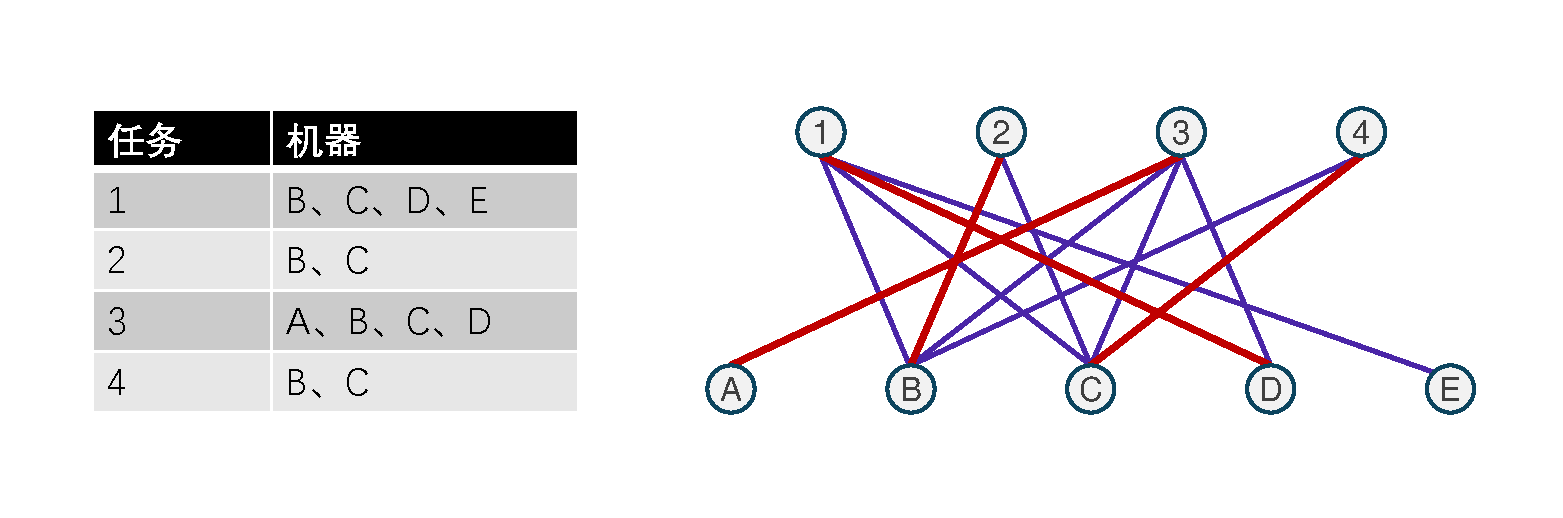
\includegraphics[width=\columnwidth]{Img/A&G.pdf}
    \bicaption {AllDifferent约束和其二部图表示。} {AllDifferent constraint and its bipartite graph representation.}
    \label{fig:AandG}
\end{figure*}

\begin{example}
    假设有四个任务(1,2,3和4)要被分配给五台机器(A,B,C,D和E)。每台机器最多只能分配一个任务,但并非每个任务都能分配给每台机器。图\ref{fig:AandG}左中展示了可能的组合,例如,任务2可以分配给机器B和C。
    由于任务必须分配给不同的机器,可以使用AllDifferent约束表述该问题,从而将问题建模为CSP。具体地,引入一个变量$x_i$,用于表示任务$i = 1, \dots, 4$,其赋值代表任务$i$被分配到的机器。变量的初始值域为图\ref{fig:AandG}左表示的任务和机器之间可能的组合,下式是构造的CSP约束:
    \begin{equation*}
        \texttt {AllDifferent}(x_1, x_2, x_3, x_4).
    \end{equation*}
    其中,$x_1 \in \{B, C, D, E\}, x2 \in \{B, C\}, x_3 \in \{A, B, C, D\}, x_4 \in \{B, C\}$。
    设$X = x_1, \dots, x_n$,其值图如图\ref{fig:AandG}右所示。值图中的红粗线表示覆盖$X$的一个匹配,它对应于CSP的解,即$x_1 = D, x_2 = B, x_3 = A$和$x_4 = C$。
\end{example}

最后,本文要介绍Hall的婚配定理\cite{hall1987representatives},它是用于推导AllDifferent约束过滤算法的图论中的一个经典定理,旨在描述一个二部图存在完全匹配的必要和充分条件。
这个定理的直观解释是,如果每个女孩(A集合)都有足够多的男孩(B集合)可以选择,那么就有可能为每个女孩找到一个男孩作为配对,形成一个完全匹配,反之亦然。
接下来,本文给出AllDifferent约束语境下,该定理的形式化描述,证明略。

\begin{theorem}\label{theorem:Hall}
    约束条件$\texttt {AllDifferent}(x_1, \dots, x_n)$有解,当且仅当对于所有的$K \subseteq \{x_1, \dots, x_n\}$,下式成立:
    \begin{equation*}
        |K| \leq |D(K)|
    \end{equation*}
    
\end{theorem}

\begin{example}
    考虑如下CSP:
    \begin{equation*}
        \texttt {AllDifferent}(x_1, x_2, x_3, x_4).
    \end{equation*}
    其中,$x_1 \in \{2, 3\}, x_2 \in \{2, 3\}, x_3 \in \{1, 2, 3\}, x_4 \in \{1, 2, 3\}$。
    可见,对于任何$K \subseteq \{x_1, x_2, x_3, x_4\}$且$|K| \leq 3$,都有$|K| \leq |D(K)|$。然而,对于$K = \{x_1, x_2, x_3, x_4\}$,有$|K| > |D(K)|$。由定理\ref{theorem:Hall}可知,这个CSP没有解。
\end{example}

\subsection{AllDifferent约束的过滤算法}

前面,本文介绍了局部一致性的概念,本文以弧一致性为例介绍AllDifferent约束如何应用局部一致性,本文首先利用二元分解将AllDifferent约束分解成一组二元约束,其定义如下。

\begin{definition}[二元分解]
设C是变量$x_1, \dots, x_n$上的一个约束。C的二元分解指在$x_1, \dots, x_n$的变量对上的一组最小的二元约束$C_{dec} = \{C_1, \dots, C_k\}$(其中$k$为整数且$k > 0$),使得C的解集等于$\bigcap_{i=1}^{k} C_i$的解集。
\end{definition}

关于$\texttt {AllDifferent}(x_1, x_2, \dots, x_n)$的二元分解是
\begin{equation}
    \bigcup_{1 \leq i < j \leq n} \{xi \neq xj\}.
\end{equation}
建立二元分解上的弧一致性的过滤算法很简单:每当一个变量的域只包含一个值时,这个值就从在AllDifferent约束中出现的其他变量的值域中被移除。这个过程一直重复,直到没有更多的变化发生或者一个域变为空。通过这个算法,可以建立AllDifferent约束上的局部一致性,或者证明它是不一致的。换句话说,当一个值域包含多个元素时,就不能推理出更多的信息了。

这个算法的一个缺点是,需要$\frac{1}{2}(n^2 - n)$个不等约束来表示一个n元的AllDifferent约束,从而这种方法的最坏情况时间复杂度是$O(n^2)$。另一个更重要的缺点是信息的丢失。当二元约束集合被弧一致化时,一次只比较两个变量。而当AllDifferent约束被超弧一致化时,所有的变量都被同时考虑,这允许更强的局部一致性,下面本文给出一个简单的例子。

\begin{example}
设一个CSP包含三个变量$x_1, x_2, x_3$,其中$x_1 \in \{2, 3\}, x_2 \in \{2, 3\}, x_3 \in \{1, 2, 3\}$。对于约束$\texttt {AllDifferent}(x_1, x_2, \dots, x_n)$,在不采用二元分解时,通过超弧一致性,可以删减$x_3$值域中的2和3;而对该AllDifferent约束使用二元分解时,由于约束被分解为多个二元约束,此时无法推导出任何信息。
\end{example}

前面,提到了AllDifferent约束和二部图的等价性,以及求解二部图最大匹配的方法。接下来,本文介绍一种利用二部图实现的GAC算法,它基于最大匹配和强连通分量,称为\textit{Régin算法}\cite{regin1994filtering}。算法思路是构造残差图表示AllDifferent约束,并通过在图上作图匹配删减冗余边,实现在约束上的全局一致性。

后文需要用到前面定义的CSP的一些概念,为了方便后文叙述,本文额外引入几个新定义。
约束$c$的\textit{变量集}是它所限制的有序变量集,记作$X(c) = \{x_1, x_2, \dots, x_r\}$。$c$的\textit{值域}是$X(c)$的值域的并集,记作$D(c) = \bigcup_{x \in X(c)} D(x)$。此外,本文使用$B_c(a)$来表示$X(c)$中值域包含$a$的变量集(即,$B_c(a) = \{x | x \in X(c), a \in D(x)\}$)。
在AllDifferent约束表示的二部图中,\textit{冗余边}指在任何最大匹配中都不出现的边。\textit{允许边}则表示属于一些但不一定所有最大匹配的边,冗余边和允许边是互补的。

一个节点是允许的,当且仅当对于一个任意的最大匹配$M$,它可以通过一个从自由节点开始的偶数交替路径到达。交替路径中的变量节点集被记为$\Gamma$,其值节点集被记为$A$。
关于允许边有如下定理,证明略。

\begin{theorem}
    一个AllDifferent约束是GAC的,当且仅当它的值图的每个边都是允许边,也即属于在$B(c)$中覆盖$X(c)$的一些匹配。
\end{theorem}

\begin{theorem}[\textbf{Berge定理}]
    一个边是允许的,当且仅当,对于一个任意的最大匹配$M$,它属于从自由节点开始的偶数增广路径或者偶数交替路径。
\end{theorem}

基于上述定理,Régin提出了执行GAC的第一个AllDifferent约束算法,通过从值图中移除冗余边来实现GAC。
该算法首先计算一组AllDifferent约束的值图的最大匹配,通过引入新的节点和将边改为有向边,构造\textit{残差有向图}如下。

\begin{definition}[\textbf{残差有向图}]
    残余有向图被定义为$R = \langle V_R, E_R \rangle$,其中$V_R = X(c) \cup D(c) \cup \{t\}$,$t$是与$D(c)$连接的一个新引入的汇节点,$E_R = E_M \cup E_U \cup E_{t_1} \cup E_{t_2}$。具体来说,每个边$e \in E_M \cup E_U$表示约束$c$中的一个变量-值对。匹配边$E_M$将变量连接到它们各自的匹配值:$E_M = \{x \rightarrow a | x \in X(c), a = M(x)\}$。未匹配的边$E_U$将值连接到它们各自的未匹配变量:$E_U = \{a \rightarrow x | a \in D(c), x \in B_c(a) \setminus \{M (a)\}\}$。$E_{t_1}$中的边将匹配值节点连接到$t$:$E_{t_1} = \{a \rightarrow t | M (a) \in X(c)\}$。$E_{t_2}$中的边将$t$连接到未匹配的值节点(自由节点):$E_{t_2} = \{t \rightarrow a | M (a) \notin X(c)\}$。
\end{definition}

通过残差有向图,可以发现,通过引入汇节点$t$,从自由节点开始的偶数增广路径被扩展为偶数的交替路径,从而允许边表现为残差图上的交替路径。
此外,很容易发现,交替路径上的顶点之间的其他边也可以扩展成一个交替路径,因此也属于允许边。从而得到如下定理:
\begin{theorem}
    一个非匹配边是允许的,当且仅当其顶点处于同一个强连通分量中。
\end{theorem}
因此,算法会计算残差有向图的强连通分量(SCC),这是算法最耗时的部分,通常通过Tarjan算法来解决。之后会删除两个端点处于不同强连通分量的非匹配边。图\ref{fig:Residual}展示了一个简单的值图转换为残差图的例子,在右图中每个框表示一个SCC,而紫红色的线段就是应当被删除的冗余边。

\begin{figure*}[t]
    \centering
    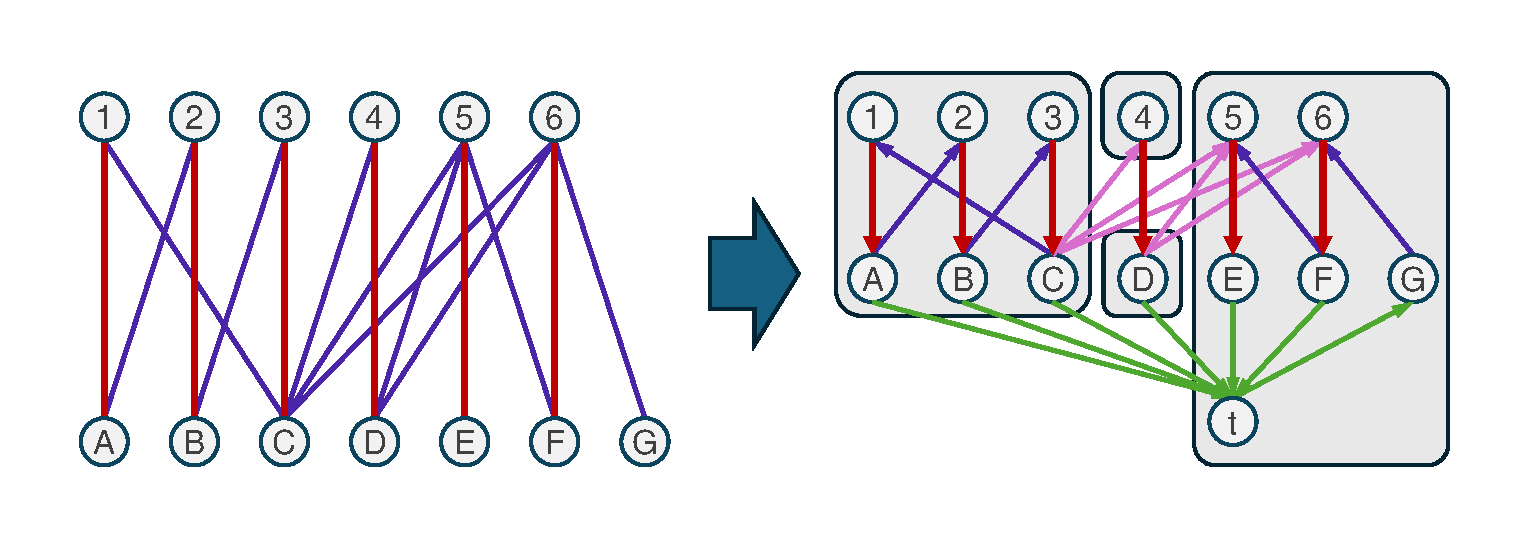
\includegraphics[width=\columnwidth]{Img/Residual.pdf}
    \bicaption {值图与残差有向图的转换。} {Value graph to residual directed graph transformation.}
    \label{fig:Residual}
\end{figure*}

近几年,有许多基于该算法的改进工作,主要思路是减少或避免SCC的计算。例如:SCC-分割\cite{gent2008generalised},它只计算在回溯搜索过程中其变量的域已经改变的SCC,从而减少了计算SCCs所需的变量范围;
匹配优化\cite{zhang2018fast},它证明了冗余边可以分为两类,其中一类可以直接删除,无需计算相应的SCCs;
早期检测\cite{zhang2021early},它避免了计算那些删除后不会分割当前SCCs的无关紧要的边;
在文献\cite{li2023bitwise}中,证明了二部图中的所有冗余边都指向某些交错环,从而对值进行筛选;
在文献\cite{zhen2023eliminating}中,发现GAC算法只关心图模型的一个节点是否在SCC中,而不是它属于哪个SCC,从而使用比特位提高算法的性能。

\section{局部搜索算法现状}

局部搜索是相对于完备搜索来说的,它是一种用于解决优化问题的常用启发式策略,而几乎所有问题都可以看作是一类优化问题,例如组合优化问题。
局部搜索的基本思想是从一个初始状态开始,然后在解的邻域中寻找更好的状态,通过一系列的移动来改进当前解。一些基本的概念的定义如下。

\begin{definition}[\textbf{状态}] 状态是解空间中的一个元素,表示问题的一个可能解。\end{definition}

\begin{definition}[\textbf{移动}] 移动是从当前状态转移到邻域中的另一个状态的操作。 \end{definition}

\begin{definition}[\textbf{打分函数}] 打分函数(评价函数)是一个将解空间中的每个状态映射到实数的函数,用于评估每个状态的优劣,即解的质量。 \end{definition}

\begin{definition}[\textbf{邻域}] 邻域是一个状态执行一次移动后的所有可达状态的集合。\end{definition}

% \begin{example}
%     设有一个旅行销售员问题,包含四个城市A、B、C和D。一个可能的状态(路径)是ABCD。如果我们交换B和C的顺序,我们就进行了一个移动,并得到一个新状态ACBD。这个状态就是原状态的邻域中的一个元素。 
% \end{example}

为了实施局部搜索算法,首先需要明确候选解的邻域结构,即确定哪些候选解可以被视为邻居。一旦邻域结构被定义,问题的解空间就可以被视为一个图形结构。因此,局部搜索实际是在图论问题上求解。以下是其求解流程:
\begin{enumerate}
    \item 设 $S = \{s_1, s_2, \ldots, s_n\}$ 为所有候选解构成的解空间,也即状态空间。
    \item 定义初始状态 $s_0 \in S$,一般由构造的初始化函数得到。
    \item 定义邻域函数 $N : S \rightarrow \mathcal{P}(S)$,将每个状态映射到其邻域的状态集合。
    \item 定义目标函数 $f : S \rightarrow \mathbb{R}$,用于评估每个状态的好坏,即解的质量。
    \item 设置停止条件,当满足某个特定条件时终止算法。常见的停止条件如达到最大迭代次数、最大时间限制等。
    \item 由打分函数(可能多个)构成移动规则,指导从当前状态的邻域中选择下一个状态。一般选择使得目标函数变好最多的状态。
    \item 从初始状态 $s_0$ 开始,按照移动规则在邻域中选择下一个状态,更新当前状态。重复这个过程,直到达到最优解或满足其他停止条件。
\end{enumerate}

若将被满足的约束数量作为最小化目标,则CSP可以被看作组合优化问题,通过局部搜索,寻找使得CSP中一致约束最多的赋值。本文以一个简单的CSP为例,介绍上面提到的概念和算法流程。

\begin{example}
假设有一个简单的约束满足问题(CSP),其中有三个变量 $X = \{x_1, x_2, x_3\}$,每个变量的取值范围是 $\{1, 2, 3\}$。目标是找到一组赋值 $A = \{a_1, a_2, a_3\}$,使得所有的约束 $C = \{c_1, c_2, c_3\}$ 都被满足。在这个问题中,状态就是变量的一组赋值,比如 $s = \{2, 1, 3\}$。移动就是改变一个变量的赋值,比如从状态 $\{2, 1, 3\}$ 移动到状态 $\{2, 2, 3\}$。目标函数就是被满足的约束数量,本文希望最小化未被满足的约束数量,也就是最大化被满足的约束数量。邻域就是通过一次移动可以达到的所有状态,比如从状态 $\{2, 1, 3\}$ 可以移动到的状态有 $\{1, 1, 3\}$、$\{3, 1, 3\}$、$\{2, 2, 3\}$、$\{2, 3, 3\}$、$\{2, 1, 1\}$和$\{2, 1, 2\}$。此时从一个初始赋值开始,通过移动来最小化未满足约束的数量,直到得到可满足解。
\end{example}

近几年,局部搜索算法发展出了很多策略,这些策略可以根据问题的特性和需求进行组合,以提高局部搜索算法的效率和效果。下面是一些例子:
\begin{itemize}
    \item \textbf{禁忌搜索\cite{glover1990tabu}}:这种策略旨在避免在已经访问过的区域中陷入循环。在禁忌搜索中,会维护一个禁忌表,记录一些在近期内已经访问过的状态。当从当前状态的邻域中选择下一个状态时,禁忌表中的状态将被排除在外。
    \item \textbf{重启策略}:重启策略能够有效避免搜索过程陷入局部最优解。若如果搜索过程在一段时间内没有找到更好的解,算法会随机选择一个初始状态重新开始搜索。这样可以使搜索过程有机会探索解空间的其他区域。 
    \item \textbf{迭代局部搜索\cite{lourencco2003iterated}}:这种策略在没有达到局部最优时,持续执行迭代改进算法。当达到局部最优时,执行随机游走算法,即从当前的局部最优解出发,进行一次或多次随机的移动,以跳出当前的局部最优区域。策略的目标是搜索一系列的局部最优解,然后返回最好的一个作为结果。
    \item \textbf{解池技术}:解池技术在搜索过程中不仅保存当前最优解,还保存一些具有代表性的非最优解,这些解构成了一个解池。通常他和重启策略一起使用,在重启时,算法从解池中选择一个解执行随机游走后得到初始状态,重新开始搜索。
\end{itemize}

在近十年来,已经有不少工作采用局部搜索来对CSP问题进行求解,并帮助解决了许多此前未解决的难题,下面本文列举一些经典及最新的工作。

在文献\cite{codognet2001yet}中,作者设计了一种新的启发式算法,它利用了问题在约束和变量方面的结构,可以比全局代价函数更精确地指导搜索进行优化(例如,违反约束的数量)。
该工作在拉丁方、N皇后、全间隔等问题上进行了实验,并且取得了较好的实验结果。
在文献\cite{DBLP:journals/tec/JinH19}中,作者设计了将拉丁方问题转化为图的方法,从而将问题归约到图着色问题上,并使用遗传算法,对给定补全拉丁方实例进行求解,取得了较好的求解效率。
在文献\cite{lloyd2020antcolony}中,作者设计了针对数独问题的蚁群算法,并尝试了多种邻域的定义,算法可以在25x25阶的困难数独实例上取得高达95\%的求解成功率。
在文献\cite{pan2022fast}中,作者设计了针对性的解池技术和子代价函数,并通过高效的化简规则对CSP进行了化简,其在拉丁方问题上,可以求解绝大部分70阶的拉丁方补全问题。


\section{本章小结}

本章节介绍了CSP、AllDifferent约束的形式化定义以及主流的求解它们的算法。
在第一节中,本文介绍了CSP的求解现状,主要介绍了CP求解器,以及其他可用于求解的技术,如SAT、SMT、ILP求解器等。
在第二节中,本文介绍了ALlDifferent约束的求解现状,主要介绍了它和图匹配的关系,以及两种主流的针对该约束的过滤算法。
在第三节中,本文介绍了局部搜索算法的概念和求解流程,以及相关的各类技术。